\section{CIG: Computational\\ Intelligence in Games}\label{subsecCIG}

The CIG StarCraft RTS AI Competition is a part of the program of the IEEE Computational Intelligence in Games (CIG) conference since August 2010. In the first year, it failed to determine the winner because of unexpected crashes caused by the custom StarCraft maps. Mike Preuss and his team members organized the event from 2011 to 2013. Traditionally, open-source policy had not been enforced to the participants and the maps unknown prior to the competition day. Since 2014, the Sejong University team (led by Kyung-Joong Kim) has organized the StarCraft AI competition at the IEEE CIG conference. Table~\ref{tableCIG} shows the change of the competition settings over years.  


\begin{table}[h] 
 \caption{The running settings of CIG StarCraft AI Competition.}
 \label{tableCIG}
 \begin{center}
 \begin{tabular} {| c c c c |}
 \hline
 Year & TM & Open-Source & Maps \\
 \hline
 2011 & Manual play & Optional & Unknown \\
 \hline
 2012 & AIIDE TM & Optional & Unknown \\
 \hline
 2013 & Java-based TM & Optional & Unknown \\
 \hline
 2014 & AIIDE TM & Forced & Unknown \\
 \hline
 2015 & AIIDE TM & Optional & Unknown \\
 \hline
 2016 & AIIDE TM & Forced & Announced \\ 
 \hline
 2017 & AIIDE TM & Forced & Announced \\ 
 \hline   
 \end{tabular}
 \end{center}  
\end{table} 

\begin{figure}[h]
  \centering
  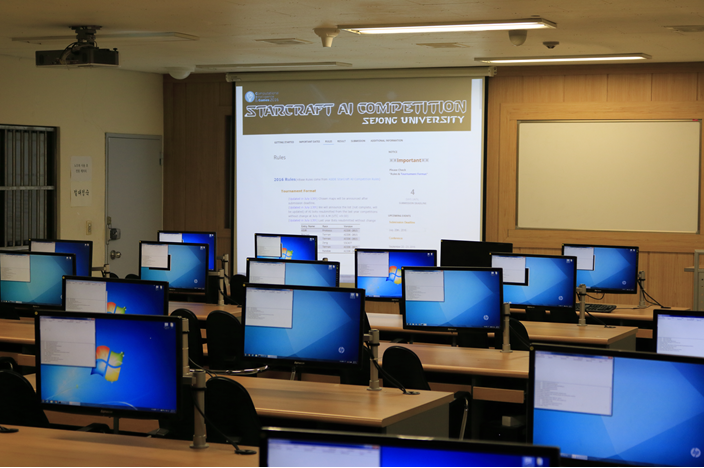
\includegraphics[width=0.5\textwidth]{fig/cig-starcraft-runs.png}
  \caption{In the computing lab, the tournament management software distributes game matches to multiple machines.}
  \label{figCIGruns}
\end{figure}

For many years, there have been changes on the selection of Tournament software, open-source policy and announcement of map pools before the competition days. Tournament management software distributes lots of matches over multiple machines on the network and automates the competition operation (Figure~\ref{figCIGruns}). Although CIG organizers developed their own JAVA-based TM sofware, the AIIDE TM has been used for the competition since 2014. Nowadays, the open-source policy is forced to the participants and all the source code is open to the public after the competition. Unlike AIIDE competition, the map pool was not known to the participants before the competition to promote generalization ability of the entries. However, we found that participants usually didn't exploit the map as a prior knowledge when they prepare the entries. After then, we announced a set of maps as candidates for the competition. 

\subsection*{CIG 2016-17 Updates \& News}\label{subsecCIGnews}

In 2016 competition, we introduced the two-stage evaluations that only half of the entries advance to the second stage based on the win ratio of the first stage. The concept of the qualification stage is not new. For example, the simulated car racing competition adopted the two-stage competitions divided into qualification stage and main race \cite{loiacono20102009}. Because StarCraft AI competition is based on the full-round robin style tournament, it's important to get high average win ratio against all other opponents. We intended to  reduce the chance that the top rankers exploit the low rankers to maximize their win ratio. 

In the second stage, it runs the competition only with the games among top rankers (top-8 players) without low-level weak players. Figure~\ref{figCIGtwostages} shows the change of rankings at the qualification and final competition. It changed the winner of the competition from Iron to TSCMOO but required additional computational resource to run the second stage. 

\begin{figure}[h]
  \centering
  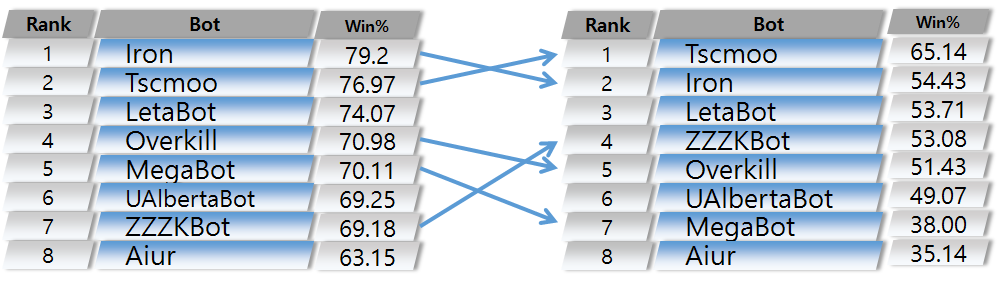
\includegraphics[width=0.5\textwidth]{fig/cig-two-stage-result.png}
  \caption{The change of the rankings at qualification (left) and main competition (right)}
  \label{figCIGtwostages}
\end{figure}

The 2016 installment of CIG competition hosted {\em 16 participants}, out of which 9 were new or updated bots and 7 were re-entries from previous year. CIG 2016 competition was divided into two stages: The {\em Qualifying} stage and the {\em Final} stage. The first qualifying stage consisted of Round Robin tournament between all 16 participating bots. In total, 11988 games were played in this stage. After the qualifying stage, best 8 bots were selected to proceed to the final stage: {\em tscmoo, IronBot, LetaBot, ZZZbot, Overkill, UAlbertaBot, MegaBot} and {\em Aiur}.

All the persistent files accumulated by the bots in the qualifying stage were deleted before entering the finals. This stage consisted of 2799 Round Robin games between the 8 bots. All the games ran on 17 computers for 8 days. The winner of the final stage, {\em tscmoo} bot created by Vegard Mella from Norway, was announced the overall winner of CIG 2016 tournament with 456 wins and $65.14\%$ win rate in the final stage. Detailed results are depicted in Figure~\ref{figCIGresults}. 

\begin{figure}[h]
  \centering
  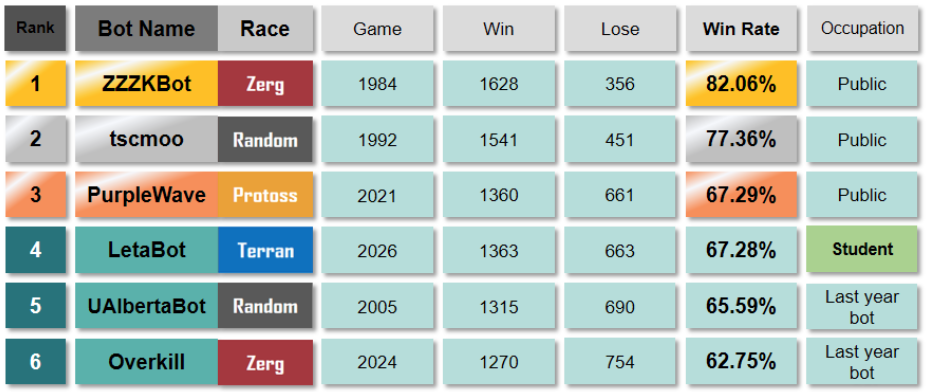
\includegraphics[width=0.5\textwidth]{fig/cig-results.png}
  \caption{Detailed results of the CIG 2016 competition final stage.}
  \label{figCIGresults}
\end{figure}

% CIG 2017 scheduled for Summer 2017
% CIG 2016 happened in Sept. 2016.  
In 2017 competition, we changed the rule from the two-stage system into the previous single round system. The reason is that the participants seem not to change their strategy to consider the two-stage style tournament. It might be interesting to adopt the SWISS-system widely used in board game community. In the setting, each player does not play against all other opponents. In the pairing, it arranges games of two players with similar scores. Usually, it produces the final outcome with relatively small number of rounds. 

In this competition, we tried to increase the number of rounds and finally reached to 125 rounds (190 games per round). Although it requires 47,500 games using 22 machines for two weeks, it helps us to understand the dynamics of AI bots' win count over rounds. Nowadays, AI bots often use multiple strategies prepared and adapt their strategies against opponents. From the long experience of gaming, they tends to know which strategy is good or bad to some opponents. The file I/O option allows them to save the game experience and reuse them to increase the chance of the wins. 

For example, Figure~\ref{figureCIGZZZTSCMOO} shows the change of the win counts over rounds for the best (ZZZKBOT) and 2nd rank players (TSCMOO). It shows that their win counts decrease after around 100 rounds. If we can continue the round-robin after the 125 rounds, the final outcome could be different because other players seem to exploit counter-strategy against the strong players. Figure~\ref{figureCIGMEGASRBOT} shows the change of the win counts for 6th rank (MEGABOT) and 14th ranker (SRBotOne). The MegaBot combined multiple AI players and selectively used them for each opponent. After 100 rounds, their win counts went up to the $75\%$. 

\begin{figure}[h]
  \centering
  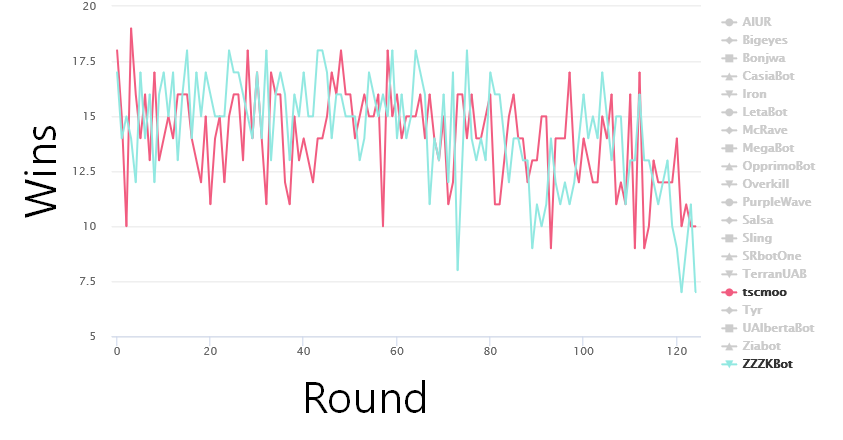
\includegraphics[width=0.5\textwidth]{fig/cig-tscmoo-zzzkbot-winrate.png}
  \caption{The change of wins over multiple rounds for ZZZKBot (1st ranker, blue), and TSCMOO (2nd ranker, red).}
  \label{figureCIGZZZTSCMOO}
\end{figure} 

\begin{figure}[h]
  \centering
  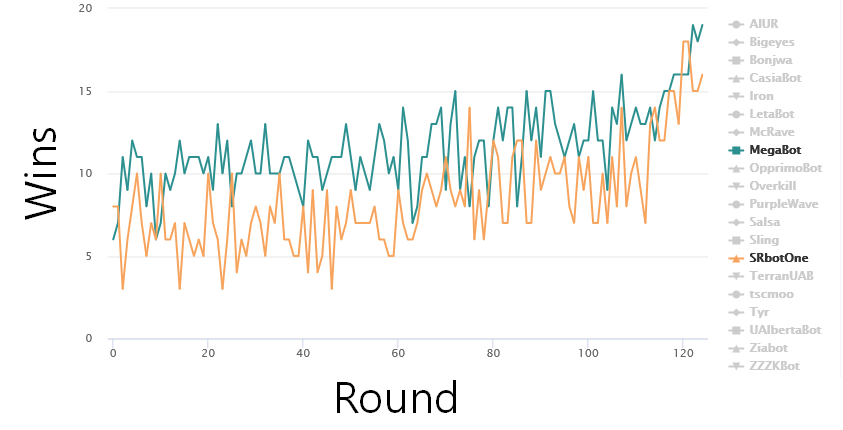
\includegraphics[width=0.5\textwidth]{fig/cig-megabot-srbotone.png}
  \caption{The change of wins over multiple rounds for MegaBot (6th ranker, blue) and SRBotOne (14th ranker, orange).}
  \label{figureCIGMEGASRBOT}
\end{figure} 


% Post-Confererence Event (Man vs. Human Match) 
After this year competition, Sejong University organized special event matches between human players and StarCraft AI players at 31st Oct 2017 (Figure~\ref{figureSong}). In the match, our university invited one novice player (ladder rating around 1100), one middle-level player (around 1500), and professional gamer, Byung-Gu Song. For the AI side, it included ZZZKBOT, the winner of CIG 2017 competition, TSCMOO, 2nd ranker in CIG, and MJBOT, specially designed AI for human players. The MJBOT has been developed since June 2017 by Cognition Intelligence Laboratory (leaded by Kyung-Joong Kim) to beat novice/middle-level players. 

In the event match, each human player had a single match against the AI players. In total, there were nine matches (3 human players X 3 AI players). In the first match, the novice human player won the first game against MJBOT but lost two games against ZZZKBOT, and TSCMOO. Although MJBOT lost the first game, it's nearly close to the win of the MJBOT but fail to finalize the match because of the programming bug. In the next session, the middle-level human player lost all the three games against the AI players. However, the Byung-Gu Song, a professional player won the all three games. It means that the AI players have potential to compete against novice and middle-level players, but not yet to the professional gamers. You can find the results and replay files of the matches from the website \footnote{\url{https://cilab.sejong.ac.kr/}}. 

\begin{figure}[h]
  \centering
  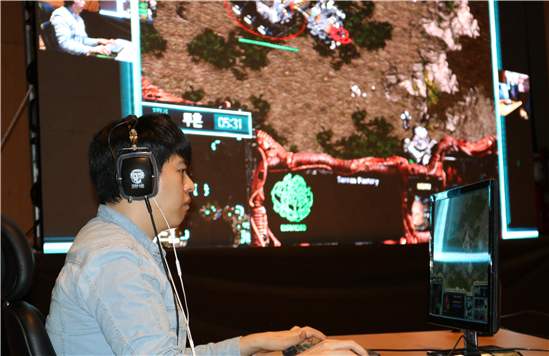
\includegraphics[width=0.5\textwidth]{fig/song_human_ai.png}
  \caption{Professional player Byung-Gu Song played against AI players.}
  \label{figureSong}
\end{figure} 
